\subsection{Sous-mission U2}

	\begin{vwcol}[widths={0.65,0.2}, rule=0pt]
	\begin{minipage}{0.7\textwidth}
	\paragraph{Objectifs de la mission}

	Mettre en valeur l'objet inconnu aparaissant sur l'image.
	\end{minipage}

	\begin{minipage}{0.3\textwidth}
	\begin{flushright}
	\paragraph{Techniques utilisées}

	Normalisation \& Detection des contours \& Isolation colorimétrique
	\end{flushright}
	\end{minipage}

	\end{vwcol} 

	\begin{figure}[h]
	\centering
		\begin{multicols}{2}
		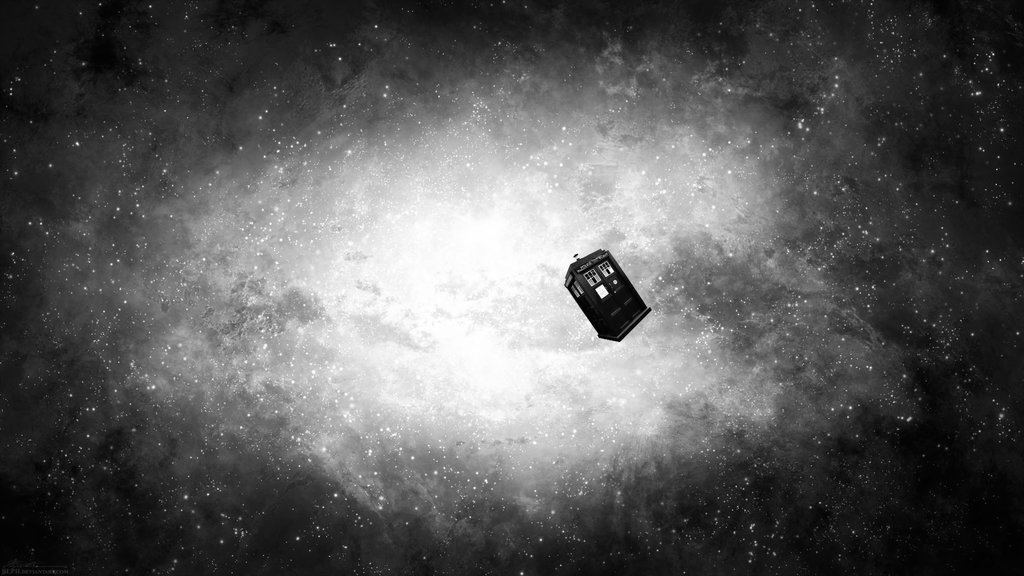
\includegraphics[scale=0.27]{images/U2_surface.png}
		Avant
		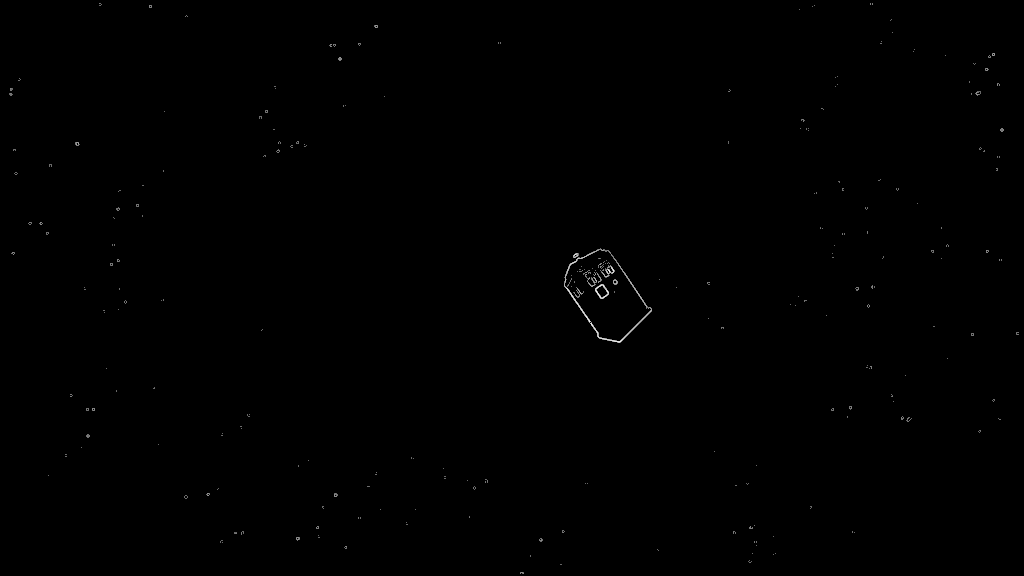
\includegraphics[scale=0.27]{images/MissionU2.png}
		Après
		\end{multicols}
	\end{figure}
	\vspace{-0.9cm}

	\paragraph{Procédé}	
		Pour mettre en valeur l'objet de l'image, nous avons tout d'abord effectué une \emph{détection de contours} sur l'image originale. Il en résulte le contour de l'OVNI. On effectue alors une \emph{normalisation} pour augmenter le contraste de l'image. Puis on sélectionne uniquement les couleurs les plus intenses pour retirer les pixels superflus.